% Welcome! This is the unofficial University of Udine beamer template.

% See README.md for more informations about this template.

% This style has been developed following the "Manuale di Stile"
% (Style Manual) of the University of Udine. You can find the
% manual here: https://www.uniud.it/it/ateneo-uniud/ateneo-uniud/identita-visiva/manuali-immagine-stile/manuale-stile

% Note: for some reason, the RGB values specified in the manual
% do NOT render correctly in Beamer, so they have been redefined
% for this document using the high level chromo-optic deep neural 
% quantistic technology offered by Microsoft Paint's color picker.

% We defined four theme colors: UniBrown, UniBlue, UniGold
% and UniOrange. For example, to write some uniud-brownish
% text, just use: \textcolor{UniBrown}{Hello!}

% Note that [usenames,dvipsnames] is MANDATORY due to compatibility
% issues between tikz and xcolor packages.

\documentclass[usenames,dvipsnames]{beamer}
\usepackage[utf8]{inputenc}
\usepackage{verbatim}
\usepackage{amsmath}
\usepackage{algpseudocode}
\usepackage{algorithm}% http://ctan.org/pkg/algorithm

\usetheme{uniud}
\graphicspath{ {./graphics/} }
\usepackage{mathtools}

%%% Bibliography
\usepackage[style=numeric,backend=biber]{biblatex}
\addbibresource{bibliography.bib}

% Author names in publication list are consistent 
% i.e. name1 surname1, name2 surname2
% See https://tex.stackexchange.com/questions/106914/biblatex-does-not-reverse-the-first-and-last-names-of-the-second-author
\DeclareNameAlias{author}{given-family}

%%% Suppress biblatex annoying warning
\usepackage{silence}
\WarningFilter{biblatex}{Patching footnotes failed}

%%% Some useful commands
% pdf-friendly newline in links
\newcommand{\pdfnewline}{\texorpdfstring{\newline}{ }} 
% Fill the vertical space in a slide (to put text at the bottom)
\newcommand{\framefill}{\vskip0pt plus 1filll}

\algdef{SE}[SUBALG]{Indent}{EndIndent}{}{\algorithmicend\ }%
\algtext*{Indent}
\algtext*{EndIndent}


\title[Support Vector Machines]{Support Vector Machines and their use in IR}
\date[May 2023]{May x, 2023}
\author[Lorenzo Zanolin]{
  Lorenzo Zanolin.
  \pdfnewline\texttt{lorenzo.zanolin@spes.uniud.it}
}
\institute{Department of Mathematics, University of Udine}

\begin{document}

\begin{frame}\titlepage\end{frame}

\begin{frame}{Outline}
\tableofcontents
\end{frame}

\section{SVM over linearly separable data}

\begin{frame}{Vector Space}
    
    \only<1->{Suppose you have to classify whether a document is \textit{relevant} or not. We can think to use \textit{terms} as features to divide properly the data. We will use a \textit{t-dimensional} vector space to represent our documents.}
    \uncover<2->{\begin{figure}[b]
        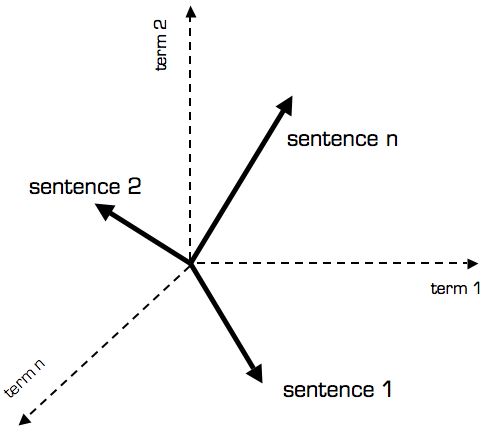
\includegraphics[scale=0.35]{graphics/vector-space.png}
    \end{figure}}
\end{frame}

\begin{frame}{Classification}
    \only<1->{For simplicity, we can reason using a 2D Space.\\ Data can be separated using a \textit{decision boundary}, which is an \textit{hyperplane}. }

    \only<1>{
        \begin{figure}[b]
            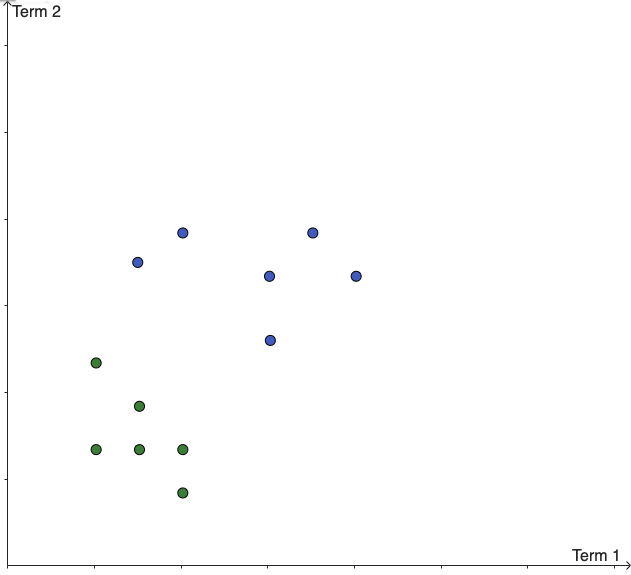
\includegraphics[scale=0.20]{graphics/before.png}
        \end{figure}}
        
    \hspace{-0.17em}
    
    \only<2>{
        \begin{figure}[b]
            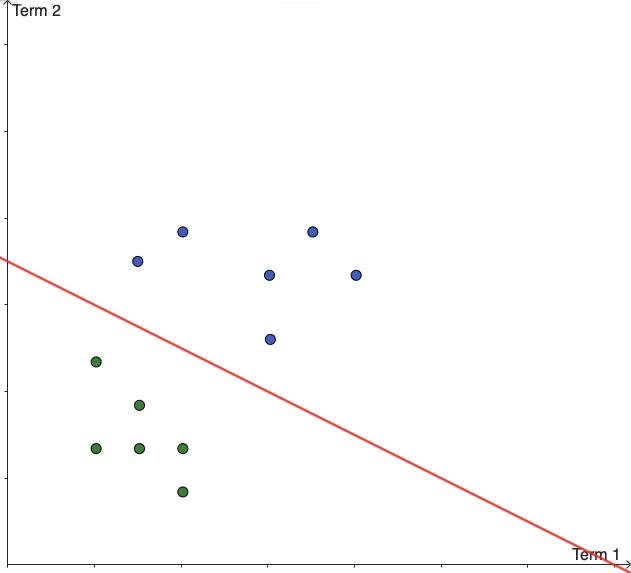
\includegraphics[scale=0.20]{graphics/after.png}
        \end{figure}}

    \hspace{-0.17em}
    
\end{frame}


\begin{frame}{Support Vectors}
    \only<1->{In the previous example the \textit{decision boundary} is a line, represented by the equation~$a + b{t}_{1} + c{t}_{2} = 0$.\\  
    We can introduce two \textit{parallels} hyperplanes (lines) to the decision boundary, called \textit{support vectors} whose equations are} 
    \only<1->{
    \begin{equation}
        \begin{cases}
          a + b{t}_{1} + c{t}_{2} = 1\\
          a + b{t}_{1} + c{t}_{2} = -1\\
        \end{cases}\
    \end{equation}}

    \uncover<2->{
        \begin{figure}[]
            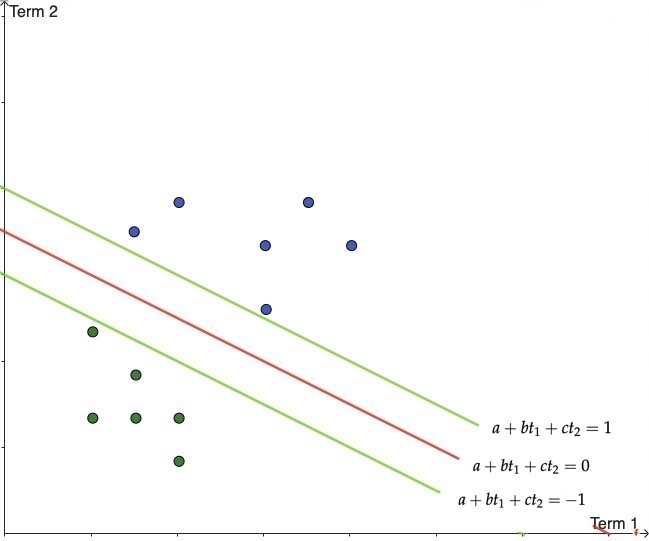
\includegraphics[scale=0.20]{graphics/support vectors.jpg}
        \end{figure}}
    \hspace{-0.1em}
    
\end{frame}

\begin{frame}{Margin}
    \only<1->{For convenience, we can rewrite the three equations using \textit{vectorization} notation.  
    \begin{equation}
        \begin{cases}
          {b}^{T}t + a = 0\\
          {b}^{T}t + a = \pm1\\
        \end{cases}\
    \end{equation}}
    
    \uncover<2->{Intuitively, we can define the \textit{margin} of the two support vectors as the distance between them.\\}
    \vspace{5mm} %5mm vertical space
    \uncover<3->{ Consider an arbitrary point $x_1$ that lies on support vector $s_1$.\\ Since $s_1,s_2$ are parallel, consider the closest point to $x_1$ belonging to $s_2$, say $x_2$.}
    \vspace{5mm} %5mm vertical space
     
\end{frame}

\begin{frame}{Margin}
    \only<1->{
        \begin{figure}[b]
            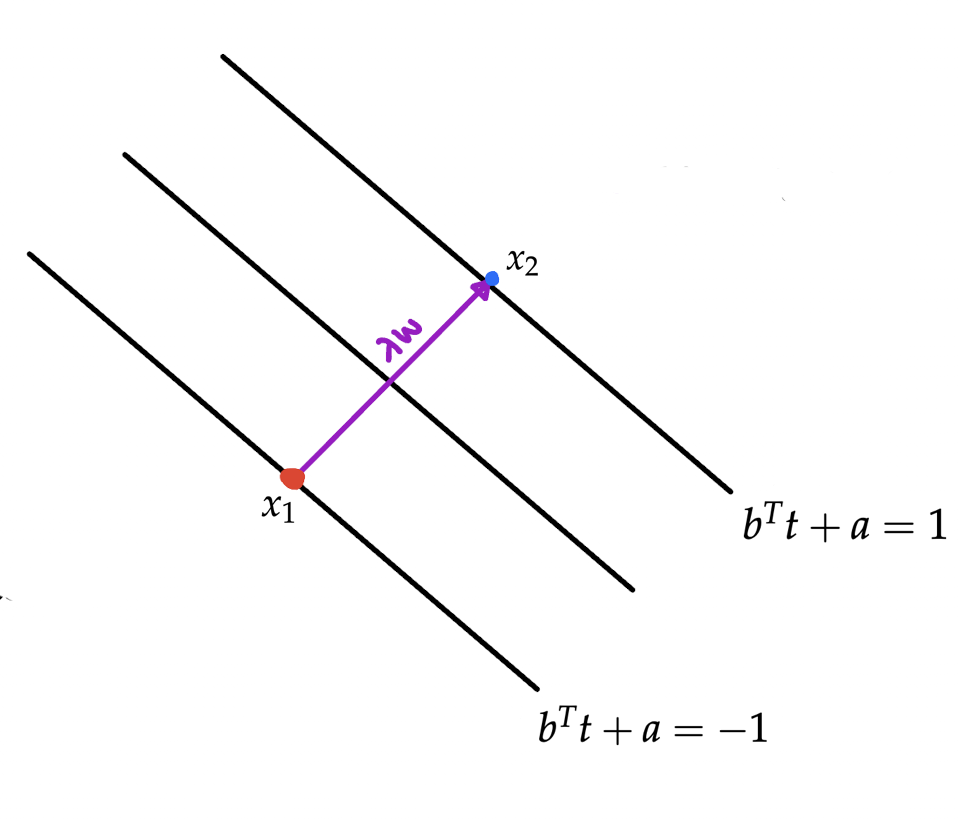
\includegraphics[scale=0.25]{graphics/distance.png}
        \end{figure}
    }
    \uncover<2->{Their distance is~$\lambda\lVert b \rVert = \frac{2}{\sqrt{{b}^{T}b}}$.\\
    \vspace{5mm}
    Vector $\lambda b$ represents the distance between the two margins.}
    \vspace{5mm} %5mm vertical space
    \uncover<3->{
    SVM~\cite{tut,svm} are used to find the \textit{maximum margin linear classifier}, thus we want to maximize the margin.}
    \vspace{5mm}

\end{frame}

\begin{frame}{Cost Function}
    \only<1->{Remembering that we want to classify documents, our goal is to find specific $b$ s.t.
    given a document $x$ belonging to class $y$ the decision boundary behaves as follows:
    \begin{equation}
        \begin{cases}
          {b}^{T}x + a \geq 1\qquad if\ y = 1\\
          {b}^{T}x + a \leq -1\qquad if\ y = -1\\
        \end{cases}\
    \end{equation}}
    \uncover<2->{We can define the \textit{cost function} as a system of equations:
    \begin{equation}
        \begin{cases}
          \min_{b,a} \frac{\sqrt{{b}^{T}b}}{2}\\
          subject\ to \quad y_i(b^{T}x_i + a)\geq1 \quad \forall x_i\\
        \end{cases}\
    \end{equation}}
     
\end{frame}

\begin{frame}{Soft-Margin}
    \only<1->{In real world problem it is not likely to get an exactly separate line dividing the data within the space. It would be better for the smooth boundary to ignore few data points than be curved or go in loops, around the outliers.\\}
    \vspace{5mm}
    \uncover<2->{So, we will use \textit{slack variables} to introduce a penalty for each misclassified point.\\}
    \vspace{5mm}
    \uncover<3>{The new cost function will be
        \begin{equation}
            \begin{cases}
              \min_{b,a} \frac{\sqrt{{b}^{T}b}}{2} + C  \sum_{i} \xi_i\\
              subject\ to \quad y_i(b^{T}x_i + a)\geq1-\xi_i\quad and\ \xi_i>0 \quad \forall x_i\\
            \end{cases}\
        \end{equation}
    Intuitively, $C$ represents how much the penalty counts.
    }
\end{frame}

\begin{frame}{Visualization}
    \only<1->{The larger is C the stricter the classification is, since a larger C will give more evidence to slack variables.
        \begin{equation}
                \begin{cases}
                  \min_{b,a} \frac{\sqrt{{b}^{T}b}}{2} + C  \sum_{i} \xi_i\\
                  subject\ to \quad y_i(b^{T}x_i + a)\geq1-\xi_i\quad and\ \xi_i>0 \quad \forall x_i\\
                \end{cases}\
            \end{equation}
    }
    \uncover<2->{
        \begin{figure}[b]
            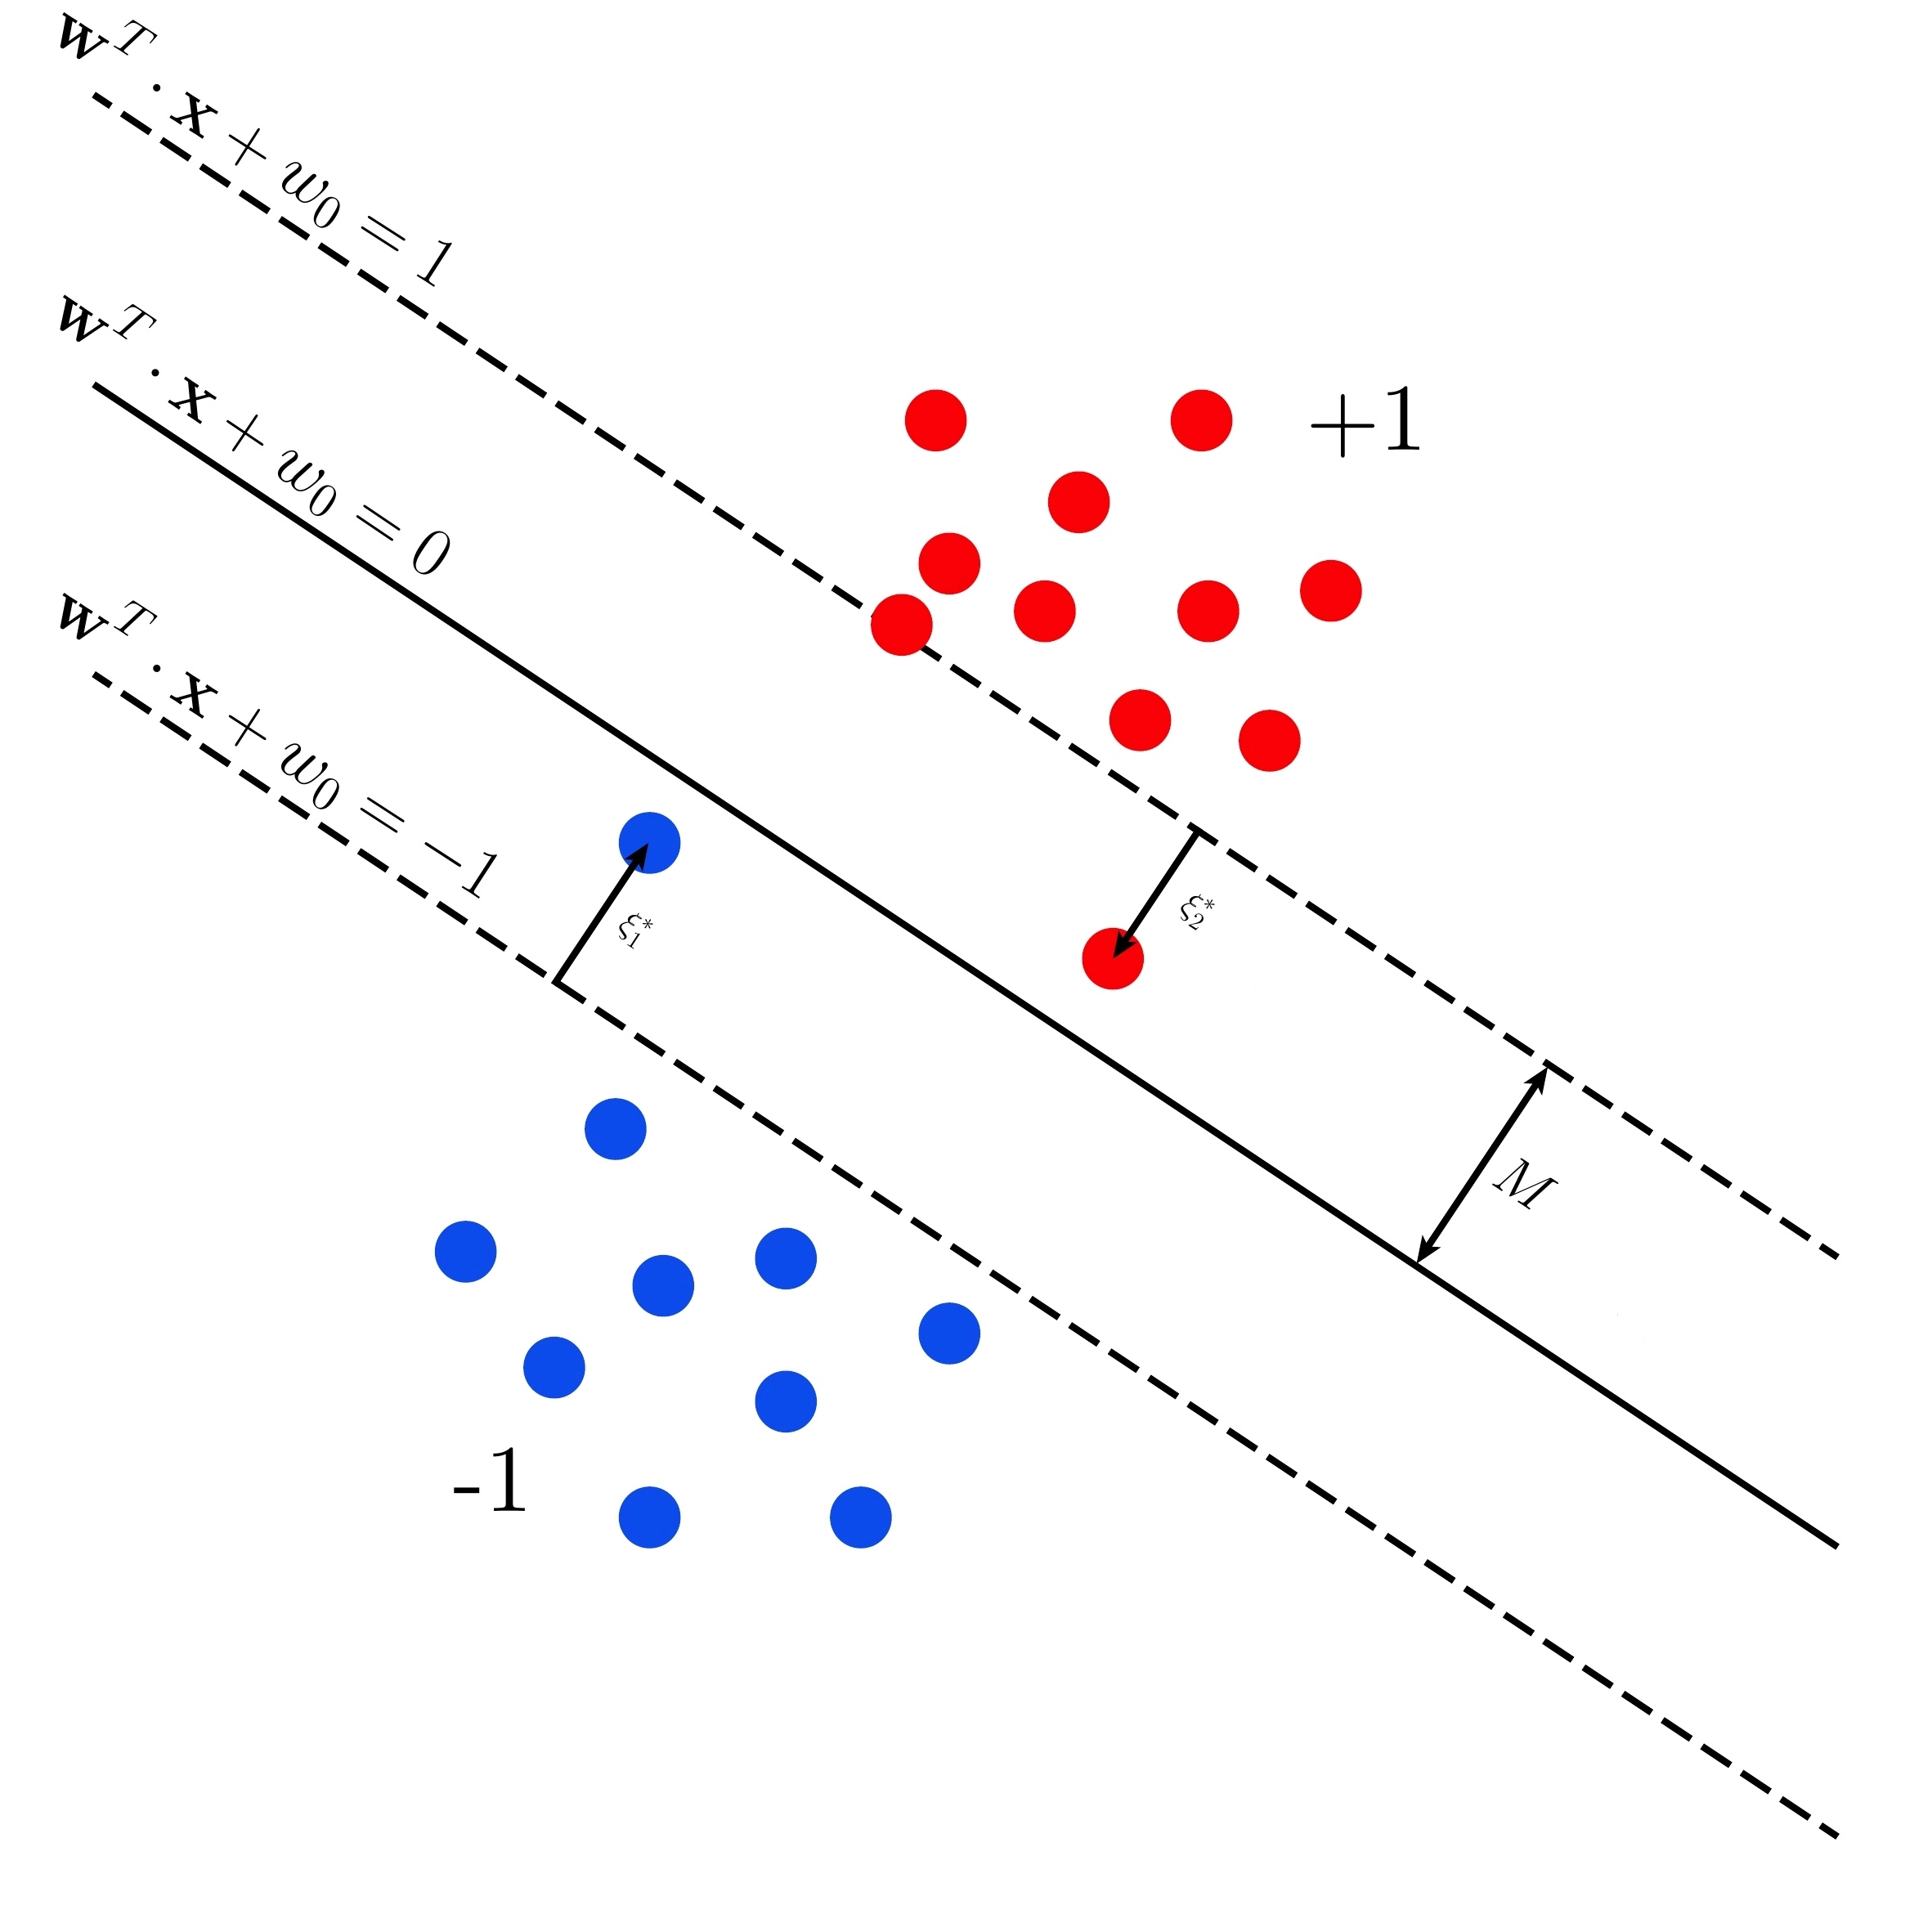
\includegraphics[scale=0.055]{graphics/slack.jpg}
        \end{figure}
    }
\end{frame}

\section{SVM over non linearly separable data}

\begin{frame}{Non linearly separable data}
    \only<1->{What if our data is not linearly separable?}
    \uncover<2->{
     It should be better to reason in a bigger dimensional space.
     \begin{figure}[]
            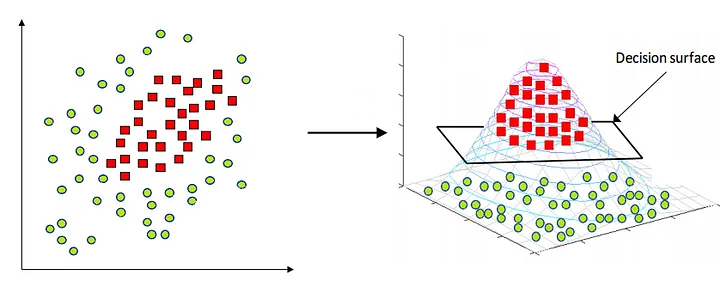
\includegraphics[scale=0.4]{graphics/kernel.jpg}
        \end{figure}
    }
    \uncover<3>{
    But augmenting dimensions costs a lot\ldots
    }
\end{frame}

\begin{frame}{Kernel Trick}
    
    \uncover<1->{Consider the function $\phi : \mathbb{R}^3 \mapsto \mathbb{R}^{10}$ used to map points in a new vector space. Calculating the \textit{similarity} ${\phi(x_i)}^T\phi(x_j)$ between each point may be intractable.\\}
    \vspace{5mm}
    \uncover<2->{Here \textit{Kernel Trick}~\cite{kernel} comes handy.\\}
    \uncover<3->{It consists of a simple linear algebra reformulation, 
        \begin{equation}
            {\phi(x_i)}^{T}\phi(x_j) = K(x_i,x_j) = {(1+{x_i}^{T}x_j)}^2.
        \end{equation}\\
    }
    \uncover<4->{
        $K$ is a \textit{kernel function} that operates on the lower dimension vectors $x_i$ and $x_j$ to produce a value equivalent to the dot- product of the higher-dimensional vectors.\\
    }
    \vspace{5mm}
    \uncover<4->{Instead of doing the complex computations in the 10-dimensional space, we reach the same result within the 3-dimensional space by calculating the dot product.}


    \vspace{5mm}
    
\end{frame}

\begin{frame}{Gaussian Kernel}
    \only<1->{There are lots of Kernel functions, an example is the \textit{Gaussian}.\\}
    \vspace{5mm}
    \uncover<2->{The idea behind is to use all $n$ training points as \textit{landmarks}.\\ Then we can calculate the similarities of each point and all the landmarks.\\}
    \uncover<3->{\begin{equation}
        \forall l_i\ similarity(x,l^{(i)}) = \exp(-\frac{{\lVert x - l^{(i)} \rVert}^2}{2\sigma^{2}})
    \end{equation}\\}
    \vspace{5mm}
    \uncover<4>{The result will be a mapping for each point in a n-dimensional space. Finally, we can identify an hyperplane which can divide correctly the two classes of points.}

\end{frame}

\section{SVM use in IR}
\begin{frame}{Pratical application}
    \only<1->{A hybrid technique used in the IR field will be presented; it uses two components: 
    \begin{itemize}
        \item \textbf{K-Means}: model for \textit{unsupervised classification};
        \item \textbf{SVM}: model for \textit{supervised classification}.
    \end{itemize}
    }
    \vspace{5mm}
    \uncover<2->{K-means algorithm is one of the most used clustering algorithms. It consists of partitioning unlabeled objects into k classes, where k is not predefined.\\ A brief explanation will follow.}
\end{frame}

\begin{frame}{K-means}
    \only<1->{The aim is to create clusters that contain \textit{similar documents}. Given a training set ${x^{(1)},x^{(2)},\ldots,x^{(m)}}$, the algorithm~\cite{kmeans} used is the following:\\}
    \uncover<2->{
        \begin{algorithm}[H]\small
            %\caption{K-Means}
            \begin{algorithmic}[1]
              \State $K\gets randomValue$  \Comment{multiple K will be tried}
              \Procedure{K-Means}{$K$}
                \State \texttt{initialize cluster centroids $\mu_1,\ldots,\mu_k$ randomly.} 
                \State \textbf{repeat until convergence\{}
                    \Indent
                    \For{$i \gets 1$ to $m$}
                        \State $c^{(i)}=arg\ min_{j} \lVert x^{(i)} - \mu_j \rVert$ \Comment{Closest centroid to $x^{(i)}$}
                    \EndFor
                    
                    \For{$k \gets 1$ to $K$}
                        \State $\mu_j = \frac{\sum_{i=1}{m} 1\{c^{(i)}=j\}x^{(i)}}{\sum_{i=1}{m} 1\{c^{(i)}=j\}}$ \Comment{New centroid of cluster $k$}
                    \EndFor
                    \EndIndent
                \State \textbf{ \} }
              \EndProcedure
            \end{algorithmic}
          \end{algorithm}
    }
\end{frame}

\begin{frame}{Visual explanation}
    \only<1>{
        \begin{figure}[]
            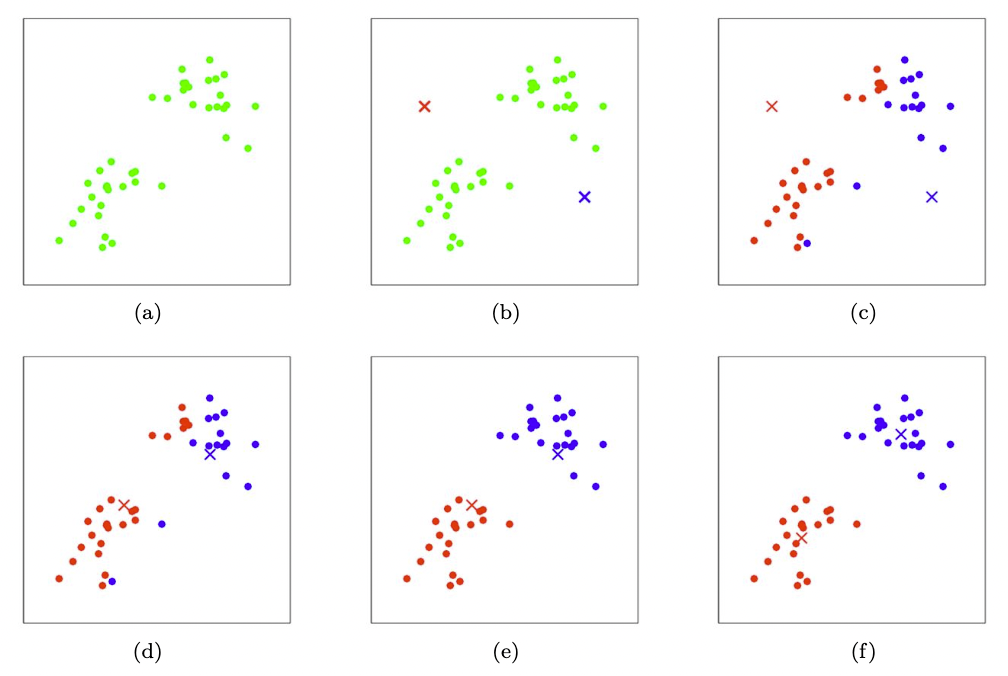
\includegraphics[scale=0.29]{graphics/k-means.png}
        \end{figure}
    }
\end{frame}

\begin{frame}{Hybrid IR System}
    \only<1->{The proposed system~\cite{hybrid} can be summarized by the following figure:}
    \uncover<2->{
        \begin{figure}[]
            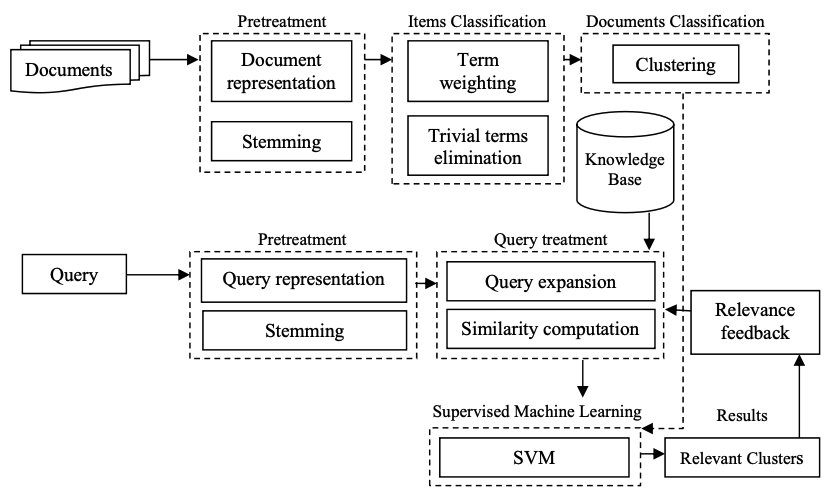
\includegraphics[scale=0.29]{graphics/hybSys entire.png}
        \end{figure}
    }

\end{frame}

\begin{frame}{Documents clustering}
    \only<1->{
        \begin{figure}[!T]
            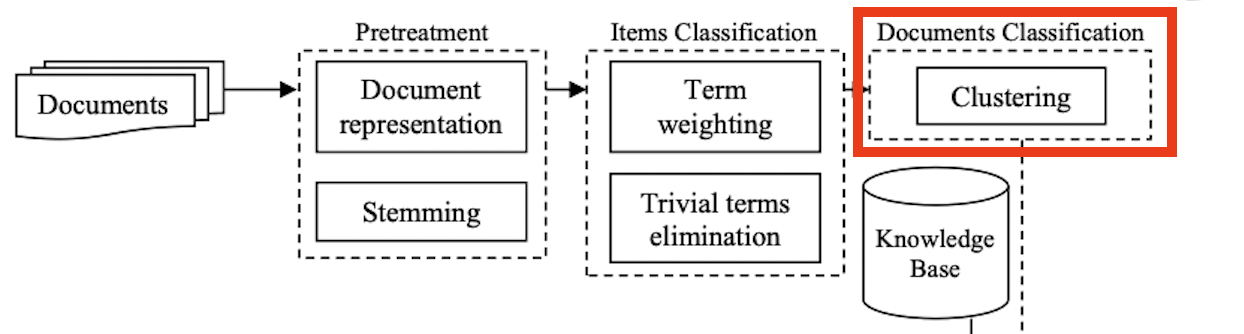
\includegraphics[scale=0.2]{graphics/hybSys top.png}
        \end{figure}
    }
    \uncover<2->{
        First part consists of text pre-processing, followed by a vector representation of each document using stemmed terms.\\ Next, there is the clustering phase.\\
    }
    \vspace{5mm}
    \uncover<3->{
        Using \textit{k-means}, documents are classified into classes of similar vectors according to the selected terms (dimensions).\\
    }
    \vspace{5mm}
    \uncover<3->{
        Finally, terms are classified as \textit{Trivial, Decisive} or \textit{Standard}. Only the last two are preserved and used as indicator of the class.
    }
    \vspace{5mm}

\end{frame}

\begin{frame}{Queries classification}

    \only<1->{
        \begin{figure}[]
            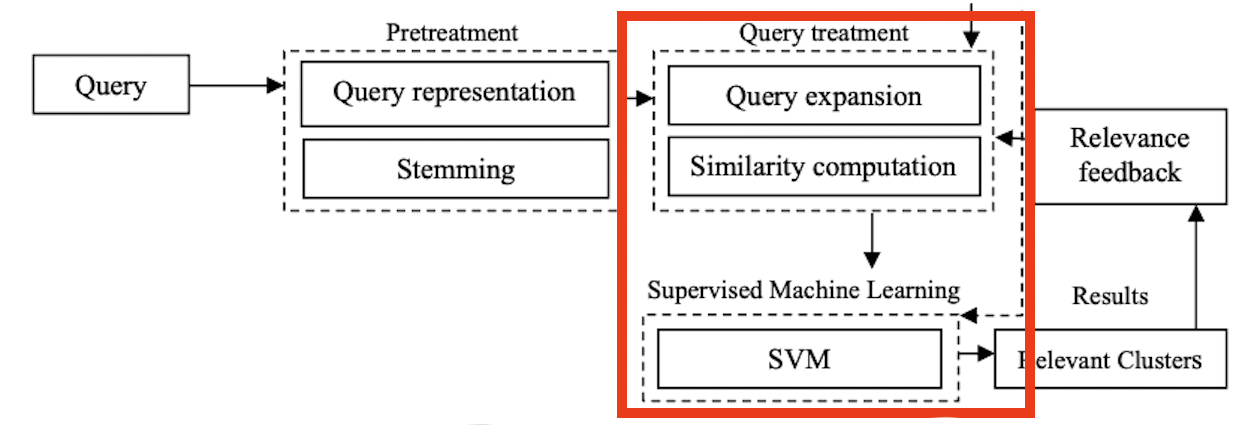
\includegraphics[scale=0.18]{graphics/hybSys bottom.png}
        \end{figure}
    }
    \uncover<2->{
        A given user query is first stemmed and represented by a vector (as for documents).\\  
    }
    \vspace{3.5mm}
    \uncover<3->{Then, SVMs are used to classify queries; for each cluster $C_i$ there will be an $SVM_i$ responsible of determining the membership of each query $q_j$ to it (giving a probability $p_i$).\\}
    \vspace{3.5mm}
    \uncover<4->{So, this process allows the selection of documents from the correct cluster (the one with the highest $p_i$).}

\end{frame}

\begin{frame}{Conclusions}

    We have seen the combination of use of SVMs and Clustering in the Information Retrieval field, with great results \cite{hybrid}.\\
    \vspace{5mm}
    To conclude, SVMs are a great tool utilized for classification and regression.\\ 
    \vspace{5mm}
    Since they are less expensive than Neural Networks, usually researchers start experimenting using them before NN.\\
    \vspace{5mm}
    
\end{frame}

\begin{frame}[allowframebreaks]{References}
    \printbibliography
\end{frame}

\end{document}